% !TeX root = ../main.tex
% -*- coding: utf-8 -*-

\chapter{基于生成对抗网络特征提取的近边界数据研究}\label{3}

DNN分类器可以由其分类边界唯一的表示,本章将讨论模型分类边界的具体表示方法,对抗性样本的可转移性及其生成近边界对抗性样本的方法和DCGAN私有化近边界数据的详细过程。

\section{近边界对抗性样本}

DNN分类器的主要工作是对数据样本进行分类,因此,一个DNN分类器的特征由其决策模式和分类边界决定。分类器的分类边界是一个抽象的概念,我们无法直接描述它,但可以根据分类器的决策结果反应分类边界。下面给出分类边界的定义:

\begin{myDef}
	\label{def:1}
	\pmb{分类边界}。给定一个数据样本$x$,如果数据样本$x$满足$g_i(x) = g_j(x)$,其中$i \neq j $并且$min(g_i(x), g_j(x)) > \mathop{max} \limits_{k \neq i, j}g_k(x)$,$g_k(x)$代表数据样本$x$被决策为类别$k$的概率,那么称数据样本$x$位于类别$i$和$j$的分类边界上。
\end{myDef}
注意,分类边界是分类器的特征,是客观存在的,和我们是否能找到这样的数据点并不相关,如何有效的找到分类边界或其附近的数据点,是本文方法要解决的问题之一。

模型窃取攻击一般会对源模型进行一定的修改,这会调整源模型的分类边界,无法保证位源模型分类边界上的样本依旧位于可疑模型分类边界上。对抗性样本是一类特殊的样本,虽然我们可以找到位于分类边界上的对抗性样本,但是在可疑模型中无法保证它们依然位于分类边界上。因此,直接利用分类边界来作为模型指纹是脆弱的。与分类边界的思想类似,本文提出了一个鲁棒性更强的近边界数据概念。下面给出近边界数据的定义:

\begin{myDef}
	\label{def:2}
	\pmb{近边界数据}。给定一个数据样本$x$,一个阈值$\theta$,如果数据样本$x$满足$\vert g_i(x) - g_j(x) \vert \leq \theta$,其中$i \neq j $并且$min(g_i(x), g_j(x)) \geq \mathop{max} \limits_{k \neq i, j}g_k(x)$,$g_k(x)$代表数据样本$x$被决策为类别$k$的概率,则数据样本$x$被称为近边界数据。
\end{myDef}

如图\ref{近边界数据示意图}所示,近边界数据位于DNN分类器的分类边界附近,距离的远近由阈值$\theta$控制。

\begin{figure}[htbp]%%图,[htbp]是浮动格式
	\centering
	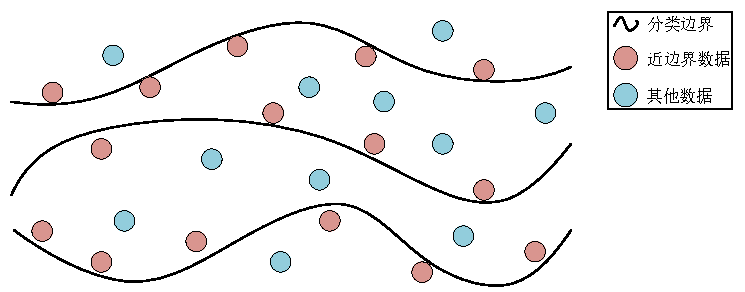
\includegraphics[width=11cm,height=7cm]{近边界数据示意图.pdf}
	%	\centerline{原始样本}
	\setlength{\abovecaptionskip}{5mm} %图片标题与图片距离
	\caption{近边界数据示意图}
	\label{近边界数据示意图}
	\end {figure}
	
相较于其他不相关的模型,对抗抗性样本可以更好的从源模型转移到其派生出的模型上。与对抗性样本类似,数据的近边界性同样在派生模型上得到保留,详细的测试结果在\ref{5}\ref{5.2}中。在下一节中,我们将讨论如何生成近边界对抗性样本。

\section{生成近边界对抗性样本}\label{3.2}

尽管近边界在模型的知识产权保护中表现出显著的效果,但是自然的近边界数据在样本空间中的占比很低,甚至可以忽略,因此如何得到一定规模的近边界数据样本仍然很困难。

根据最近的一些研究\cite{cao2021ipguard},对抗性样本通常被用于确定分类器的分类边界。具体而言,对抗性样本有两个分类:原始分类和目标分类。其中,原始分类是该样本不经过特殊处理的原始分类结果,目标分类是对原始样本添加微小噪声后的分类结果。如图\ref{原始样本与对抗性样本对比}所示,对抗性样本对分类边界的跨越体现在,在视觉上对抗性样本和原始样本几乎没有差别,但是分类结果却是目标分类。

\begin{figure}[htbp]%%图,[htbp]是浮动格式
	\begin{minipage}[t]{0.49\linewidth}        %图片占用一行宽度的50%
		\hspace{2mm}
		\centering
		
\includegraphics[width=5cm,height=3.5cm]{对抗性样本原图.jpg}
		\centerline{(a)原始样本}
	\end{minipage}
	\begin{minipage}[t]{0.49\linewidth}        %图片占用一行宽度的50%
		\hspace{2mm}
		\centering
		
\includegraphics[width=5cm,height=3.5cm]{对抗性样本.jpg}
		\centerline{(b)对抗性样本}
	\end{minipage}
\setlength{\abovecaptionskip}{7mm} %图片标题与图片距离
\caption{原始样本与对抗性样本对比}
\label{原始样本与对抗性样本对比}
\end {figure}


本文认为该特征可以帮助获得较多的近边界数据,具体来说,我们将从大量的对抗性样本中挑选近边界数据。因此,本文测试了几种常用的生成对抗性样本的方法,以帮助我们构建近边界数据。测试过程中,不同方法的优劣取决于生成对抗性样本到分类边界距离的远近,距离近者更优。在定义\ref{def:2}的基础上,下面给出量化的距离定义:

\begin{myDef}
	\label{def:3}
	\pmb{分类边界距离}。给定一个数据样本$x$,它到分类边界的距离$distance = \vert g_i(x) - g_j(x) \vert$,其中$i \neq j $并且$min(g_i(x), g_j(x)) \geq \mathop{max} \limits_{k \neq i, j}g_k(x)$,$g_k(x)$代表数据样本$x$被决策为类别$k$的概率。
\end{myDef}

\noindent\textbf{Fast \ Gradient \ Sign \ Method(FGSM):}FGSM \cite{goodfellow2014explaining}是最经典的构建对抗性样本的方法之一,它是一种基于梯度生成对抗性样本的方法,属于无目标攻击方式。只需要对原始样本添加微小的扰动$\eta$,如式\ref{eq:3.1},\ref{eq:3.2}所示,即可生成样本$x$的对抗性样本$\tilde{x}$。

\begin{equation}
	\label{eq:3.1}
	\eta = \epsilon \cdot sign(\bigtriangledown_xJ(\theta,x,y^*))
\end{equation}
\begin{equation}
	\label{eq:3.2}
	\tilde{x} = clip(x + \eta)
\end{equation}

\noindent 其中$sign$是符号函数,$x$表示原始样本,$y^*$表示$x$的真实类别,$\theta$表示模型权重参数,$J$表示分类器损失函数,$\bigtriangledown_x$表示对原始样本$x$求偏导,$clip$函数是将样本投射回可行数据域,比如图像样本的像素点范围在$[0,1]$内,$\epsilon$用来控制变化幅度。

FGSM 生成对抗性样本的速度非常快,但其结果非常依赖$\epsilon$的选择,因此探索不同的$\epsilon$是使用该方法的重点。

\noindent\textbf{Iterative \ Gradient \ Sign \ Method(IGSM):}IGSM\cite{kurakin2018adversarial}是FGSM的进阶版本,如式\ref{eq:3.3},\ref{eq:3.4}所示,与FGSM只进行一次扰动叠加不同,IGSM采用迭代的形式构造对抗性样本,每次叠加一个小扰动。这个过程持续到成功生成对抗性样本或者达到迭代次数上限。

\begin{equation}
	\label{eq:3.3}
	\eta = \alpha \cdot sign(\bigtriangledown_xJ(\theta,x,y^*))
\end{equation}
\begin{equation}
	\label{eq:3.4}
	\tilde{x}_t = clip(\tilde{x}_{t - 1}  + clip_{\epsilon}(\eta))
\end{equation}

\noindent 其中$\alpha$是步长大小,$\tilde{x}_t$表示第$t$次迭代后的结果,$clip_{\epsilon}$是限定每次叠加的范围不超过$\epsilon$,其余参数与FGSM保持一致。

除此之外,我们还测试了FGSM的另一个进阶版本RFSGM\cite{tramer2017ensemble}, RFSGM增加了扰动的多样性,可以更精细地生成对抗性样本。在实际结果中我们发现尽管FGSM生成对抗性样本速度非常快,但是对抗性样本距离分类边界的距离比较远。IGSM 和RFGSM 效果要比FGSM 好,但仍认为不符合我们的期望。在大量的测试中,我们发现CW能够生成大量位于分类边界附近的样本,具体的测试结果在\ref{5}\ref{5.2}中。

\noindent\textbf{Carlini \ and \ Wagner's \ methods(CW):}CW \cite{carlini2017towards}方法是一种有目标的攻击方式,同样是添加噪声到对抗性样本中,但其具有三种变体:CW-$L_0$,CW-$L_2$和CW-$L_{\infty}$,不同的变体使用不同的方法来衡量噪声的大小,其中CW-$L_2$在实验中效果最为突出,因此本文使用该方法作为生成对抗性样本的选择。具体而言,CW-$L_2$对于给定的初始样本采用二分搜索的方式迭代搜索一个小噪声,并且每次搜索记录下最小的扰动。CW-$L_2$的损失函数如式\ref{eq:3.5},\ref{eq:3.6},\ref{eq:3.7}所示:

\begin{equation}
	\label{eq:3.5}
	Loss = Loss1 + Loss2 
\end{equation}
\begin{equation}
	\label{eq:3.6}
	Loss1 = D(x, x + \delta)
\end{equation}
\begin{equation}
	\label{eq:3.7}
	Loss2 = c \cdot f(x + \delta,target)
\end{equation}
$$s.t. \ x + \delta \in [0,1]^m$$

\noindent 其中$target$是目标标签,$c$是惩罚因子,用于权衡$Loss2$的影响大小,通过二分查找来寻找合适的$c$,$Loss1$约束对抗性样本$x + \delta$和原始样本$x$尽可能相似,$Loss2$约束对抗性样本$x + \delta$的决策结果为目标标签。

根据定义\ref{def:3},数据样本$x$距离分类边界的距离是$distance = \vert g_i(x) - g_j(x) \vert$,我们希望生成的对抗性样本距离分类边界的距离尽可能近。本文算法迭代过程中引入这一目标,改进算法迭代的过程,在保持生成对抗性样本靠近分类边界的同时,提高算法效率。具体而言,在迭代过程中,我们仅在$distance$变小时更新距离参数和对抗性样本,并在$distance$小于预定的阈值$\theta$时提前终止迭代,具体的过程如算法\ref{alg:1}所示。

\begin{algorithm}[H] 
	\setstretch{1.2}
	\caption{改进的二分查找CW-$L_2$算法}
	\label{alg:1}
	\begin{algorithmic}[1]
		
		\Require 样本$x$;模型$M$;阈值$\theta$;二分次数$n$;迭代次数$iteration$;原始标签$r$;目标标签$t$
		\Ensure 近边界对抗性样本$x'$
		\State 参数初始化:$c\gets1$,$distance \gets 1$
		\For {$i=1,2,...,n$}
			\State $isSuccessAttack \gets false$
			\State $w \gets arctanh(x)$
			\State $w\_pert \gets zero\_like(w)$
			\For{$j=1,2,...,iteration$}
				\State $new\_img \gets tanh(w + w\_pert)$
				\State $new\_distance \gets \vert g_r(new\_img) - g_t(new\_img) \vert$
				\If{$new\_distance < distance$}
					\State $distance \gets new\_distance$
					\State $x' \gets new\_img$
					\State $isSuccessAttack \gets true$
				\EndIf
				\State 使用$Adam$更新$w\_pert$
			\EndFor
			\If{$isSuccessAttack == true$}
			\State 减小$c$
			\Else \State 增大$c$
			\EndIf 
			\If{$distance \leq \theta$} 
			\State $break$
			\EndIf
		\EndFor
		\State \textbf{return} $x'$
	\end{algorithmic}
\end{algorithm}


在这一阶段,我们只是在源模型的样本空间中挑选一部分数据作为初始样本添加小噪声,针对性地生成了目标分类对抗性样本。在此阶段源模型的训练和原始数据均不受任何影响,防御者只需要针对性的生成对抗性示例即可。然而,近边界数据作为推断所有权的重要证据,直接生成对抗性样本也极易受到盗窃者的复制。因此,我们需要将生成的近边界数据私有化,具体操作将在下一节中给出。

\section{近边界数据私有化}\label{3.3}

由于通过生成对抗性样本的方法构建近边界数据这一步骤十分容易复现,并且现在大多数模型训练使用的数据都来源于公开数据。因此我们需要从公开的训练数据中构建自己私有化的近边界数据,以防止模型所有者的近边界数据被轻易模仿。在本文中,我们希望可以通过训练一种模型学习上一节中生成的近边界对抗性样本特征,并以此生成新的近边界数据。这种新的数据从视觉上不一定和原始数据类似,但其原始的特征以及添加的噪声需要被学习,并根据提取到的特征生成的新样本对于源模型同样是近边界数据。因为本文用到的是图像样本,CNN可以很好的处理图像,因此,在本文中我们设计了一种基于DCGAN\cite{radford2015unsupervised}的特征提取器,提取近边界数据的特征之后,使用生成器并生成私有化近边界数据。
%注意生成器以,$CW$-$L_2$生成的对抗性示例作为输入,并输出私有化后的近边界数据。

\begin{figure}[htbp]%%图,[htbp]是浮动格式
	\centering
	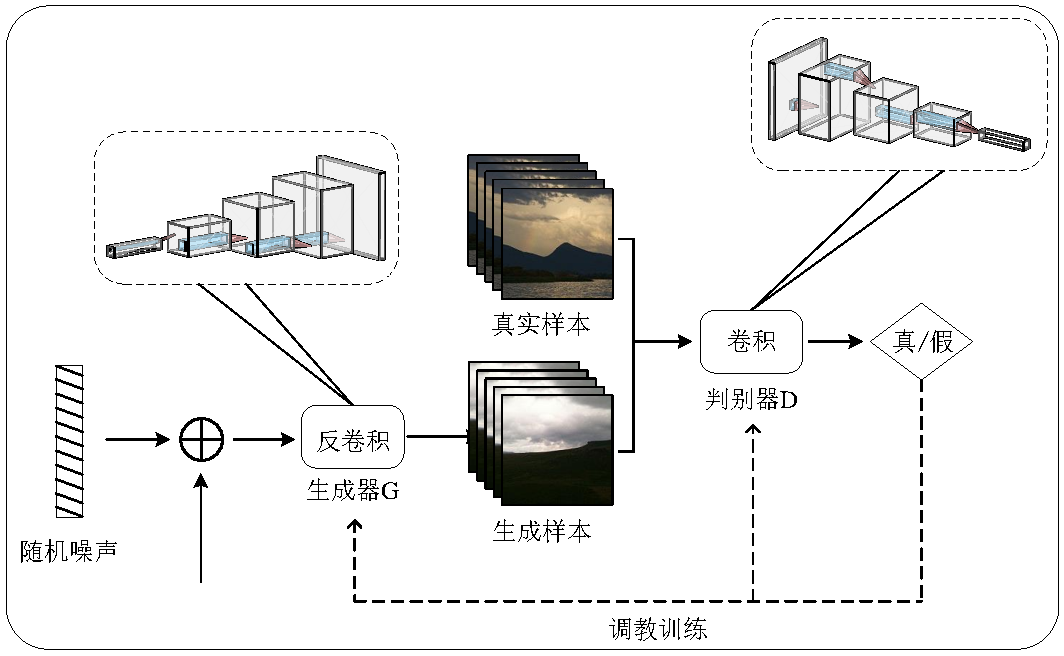
\includegraphics[width=14.5cm,height=8cm]{DCGAN网络结构图.pdf}
	%	\centerline{原始样本}
	\setlength{\abovecaptionskip}{5mm} %图片标题与图片距离
	\caption{DCGAN网络结构图}
	\label{DCGAN网络结构图}
\end {figure}

如图\ref{DCGAN网络结构图}所示,DCGAN的大体结构与训练方式和普通GAN类似,但是DCGAN将CNN与GAN相结合,生成器$G$和判定器$D$都用CNN替换原始GAN的全连接网络。得益于CNN对图像的处理能力,DCGAN极大提升了网络训练稳定性和生成样本的质量。具体而言,DCGAN主要是从网络架构上改进了原始的GAN,主要改进如下:

\begin{enumerate}
	\renewcommand{\labelenumi}{\theenumi)}
	\item DCGAN的生成器和判别器均去掉CNN的池化层,生成器使用反卷积层还原图片,判别器保留CNN的整理架构,使用卷积层提取图片特征。
	\item 在生成器和判别器中都使用Batch Normalization层,加速模型训练的同时提升训练的稳定性。
	\item 生成器除最后一层使用Tanh激活函数外,其余层使用ReLU,判别器所有层均使用LeakyReLU。
\end{enumerate}

我们希望DCGAN能够学习到足够多的近边界数据特征,尝试修改其判定器的目标函数,在保留梯度的情况下将其与源模型的结果相连,得到的结果在同样的生成规模下确实优于原始DCGAN的生成情况。然而,考虑到两者的效率,实际情况下生成的结果并无较大区别。

训练DCGAN的具体流程如算法\ref{alg:2}所示。

\begin{algorithm}[!h] 
	\setstretch{1.3}
	\caption{训练DCGAN模型}
	\label{alg:2}
	\begin{algorithmic}[1]
		
		\Require 近边界数据$\tilde{D}$;批处理大小$batchsize$;训练轮次$epoch$;损失函数$Loss$
		\Ensure 训练好的DCGAN模型
		\State 参数初始化:$learning \ rate \gets 0.0002$,$real\_label \gets 1$,$fake\_label \gets 0$
		\For{$i=1,2,...,epoch$}
		\State 随机噪声$z \gets 100$ 
		\State $x' \gets G(z)$
		\State $Loss1 \gets Loss(D(x), real\_label)$  \Comment $x$是近边界数据样本
		\State $Loss2 \gets Loss(D(x'), fake\_label)$
		\State $Loss_D \gets Loss1 + Loss2$
		\State $Loss_G \gets Loss(D(x'), real\_label)$ \Comment 生成器希望$D(x') $接近$real\_label$
		\State 使用$Adam$更新生成器$G$,判别器$D$参数
		\EndFor
	\end{algorithmic}
\end{algorithm}

尽管构建的近边界数据已经都位于目标分类边界附近,但我们仍希望近边界数据最大程度上靠近目标分类边界。近边界数据与目标分类边界的距离越近,推断模型所有权成功的可能性就越大。此外,生成的近边界数据虽然只被模型所有者拥有,但对于一些功能易被泛化的模型,近边界的特性仍有可能被泛化。因此,本文提出使用近边界数据微调源模型的目标分类边界。如式\ref{eq:3.4}所示,$Loss_{FT}$是针对目标分类边界的损失函数。

\begin{equation}
	\label{eq:3.10}
	Loss_{FT} = \frac{1}{n} \sum^{n}_{i = 1} (g_t(x_i') - g_s(x_i'))^2
\end{equation}

\noindent 其中$n$是该目标分类边界的近边界数据的数量,$x_i'$是生成的近边界数据,$g_t(\cdot)$和$g_s(\cdot)$分别表示目标分类概率和源分类概率,$Loss_{FT}$本质是希望近边界数据更靠近目标分类边界。$Loss_{FM}$是源模型的损失函数,我们设计两者交替训练微调源模型,与DCGAN 的过程相似,这是一个博弈的过程,具体的流程如算法\ref{alg:3}所示。

\begin{algorithm}[H] 
	\setstretch{1.3}
	\caption{微调源模型}
	\label{alg:3}
	\begin{algorithmic}[1]
		
		\Require 原始数据集$D$;私有化近边界数据$D'$;批处理大小$batchsize$;训练轮次$epoch$;损失函数$Loss_{FT}$,$Loss_{FM}$;源模型$M$
		\Ensure 微调后的源模型$M'$
		\State 参数初始化:$learning \ rate \gets 0.0001$
		\For{$i=1,2,...,epoch$}                          
		\State $Loss1 \gets Loss_{FT}(g_t(x') , g_s(x'))$ \Comment $g_k(x')$:$x'$在第$k$类上的概率
		\State $Loss2 \gets Loss_{FM}(M(x), label)$ \Comment $label$指正常样本的原始标签
		\State 使用$Adam$更新生成器$G$,判别器$D$参数
		\EndFor
	\end{algorithmic}
\end{algorithm}

\noindent 其中$x$指正常的样本,$x'$指DCGAN生成器生成的私有化近边界数据。
\begin{table}[h]
	\centering
	\setlength{\arrayrulewidth}{0.5mm}
	\renewcommand\arraystretch{1.8}
	\caption{微调分类边界对模型的影响}
	\label{table:state}
	\begin{tabular*}{13cm}{@{\extracolsep{\fill}} l c c}
		
		\hline
		数据集        &    微调前准确率   &   微调后准确率            \\
		\hline
		CIFAR-10      &     0.886        &     0.873               \\
		
		Heritage      &     0.879        &     0.866               \\
		
		Intel\_image  &     0.854        &     0.846               \\
		\hline		
	\end{tabular*}
\end{table}

微调目标分类边界使近边界数据与源模型之间的联系更加紧密。注意,我们只微调目标分类边界,且通过交替微调尽可能减少微调对源模型的影响,如表\ref{table:state}所示,微调前后源模型的精度差不超过3\%,因此,微调对于源模型的性能影响十分微小,甚至可以被忽略,但却有效提高了最后的所有权推断效果。更多微调目标分类边界对准确度的影响测试在\ref{5}\ref{5.4}中。


\section{本章小结}

本章主要描述了近边界数据的特性和生成近边界数据并将其私有化的过程。对抗性样本一般位于DNN模型分类边界上,并且可以很好的转移到其派生出的模型上。鉴于模型攻击一般会对源模型进行修改,本章提出了鲁棒性更强的近边界数据的概念,数据的近边界性也可以转移到其派生模型上,改变的是近边界数据到分类边界的距离。由于自然的近边界数据很少,本章对比了常见的生成对抗性样本的方法,在CW-$L_2$算法的基础上,引入了分类边界距离的概念来更快的生成近边界对抗性样本。考虑到敌手可能会产生近边界数据,我们设计了基于DCGAN的数据生成器,来私有化近边界数据,并在此基础上使用近边界数据微调源模型分类边界,提高所有权推断置信度。
